% !TEX root = thesis.tex
\chapter{考察と提言}
この章では、5章と6章の結果に対する考察を行うと共に、考察結果を踏まえ、Deep Learningの実問題における効率的な応用方法について、提言を行う。
\section{5章の実験に関する考察}

・pylearn2におけるMaxout Networkは、元論文に記されている精度こそ再現できないが、MNISTの分類タスクにおいてState of the Artに近い精度を実現することが出来た。\\
・今回の実験では、MNISTの1次元版、2次元版共に、元の論文やpylearn2ソースコードの付属テキストに書いてあった分類誤差よりも、大きい誤差しか再現できなかった。また、この誤差が大きくなってしまう問題は、複数回の実験を行っても、解決しなかった。\\
分類精度が悪くなってしまった理由として、当初、図\ref{c7_maxout_cause}に挙げた3つの原因が考えられた。しかし、複数回実行しても全く同じ結果が出たため、乱数のシードを変更しない限り、内部的には全く同じ演算が成されていると考えられる。よって、「重みのランダム初期化」、つまり「ニューラルネットワークの接続の重みがランダムに決まっており、たまたま分類に不利な重みからスタートしたため、元の論文よりも悪い結果が出てしまった」という仮説は否定される。残る可能性は、「ソースコードのバージョン」と「ハードウェア構成の違い」であるが、GPUを始めとする各パーツの性能は、元論文の実験時に使われたものよりも、今回の実験で使ったものの方が高いため、「ハードウェアの性能」に原因を求めるのも難しい。残る可能性は「ソースコードのバージョン」である。これは、pylearn2が依存しているライブラリの、numpyやscipy、Theanoまたpylearn2自体などがアップデートされたことにより、内部的に細かい計算方法が変化し、分類誤差の再現性が下がってしまった、という仮説である。これについては、Maxout Networkの元実験を行ったメンバーも、
\begin{quote}
All of pylearn2's dependencies (theano / scipy / numpy / etc.) make reproducibility
very difficult. As such, we are not currently going to make any effort to ensure that
all results are widely reproducible on a variety of platforms. Instead, we will
record the platform on which they were verified to be correct.
\end{quote}
と記している(pylearn2のソースコード\footnote{\url{pylearn2/scripts/papers/maxout/notes}}より引用)。\\
\begin{figure}[tbp]
 \begin{center}
  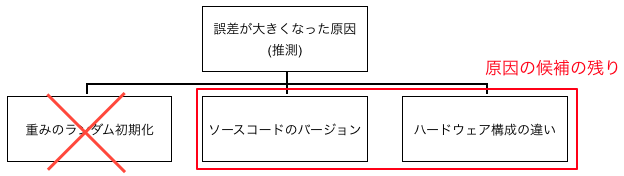
\includegraphics[width=80mm]{img/c7/maxout_error_cause}
 \end{center}
 \caption{Maxout NetworkによるMNIST分類実験で、誤差が論文より大きくなった原因}
 \label{c7_maxout_cause}
\end{figure}
・CIFAR10の実行時間が長くかかるのは必要不可欠なのか、それとも短縮する方法があるのか、検証する必要がある。\\
\section{6章の実験に関する考察}

\section{深層学習の利用法に関する提言}
・Maxout Networkが良い精度を実現できたこと、改造のしやすさ、GPU利用の簡便さなどを考え合わせると、現時点では、pylearn2を通してDeep Learningを利用するのが良いと考えられる。

高い学習性能 → Maxout Networkの1次元版で解決できる。Maxoutの実装は、 pylearn2を使うとよい
実行時間 → Theanoを通じたGPU利用で緩和できる。CPUのみのマシンでも一応 動かせる
実行プログラムの使いやすさ → モジュール化が明確で、Datasetクラスを書く だけのpylearn2が良い
アルゴリズムの改良・調整の容易さ → モジュール化が明確で、設定用のyaml ファイルを書くだけのpylearn2が良い 

Matlabやc++などで書かれたソースコードもあるが、学習性能を キープしつつ、GPU/CPUを透過的に扱えて、改良・調整も容易なpylearn2を使う と良い 
